\section{Results}
\subsection{Single-Task Classifiers}
We ran Naive Bayes and logistic regression on all 6 tasks independently and computed accuracy, precision, recall and the F1-measure of each classifier. Figure \ref{fig:naivebayes} gives all the results for the Naive Bayes classifier and Figure ... lists the logistic regression results.

%
\begin{figure}
    \centering
    \setlength{\tabcolsep}{0.0130\linewidth}
    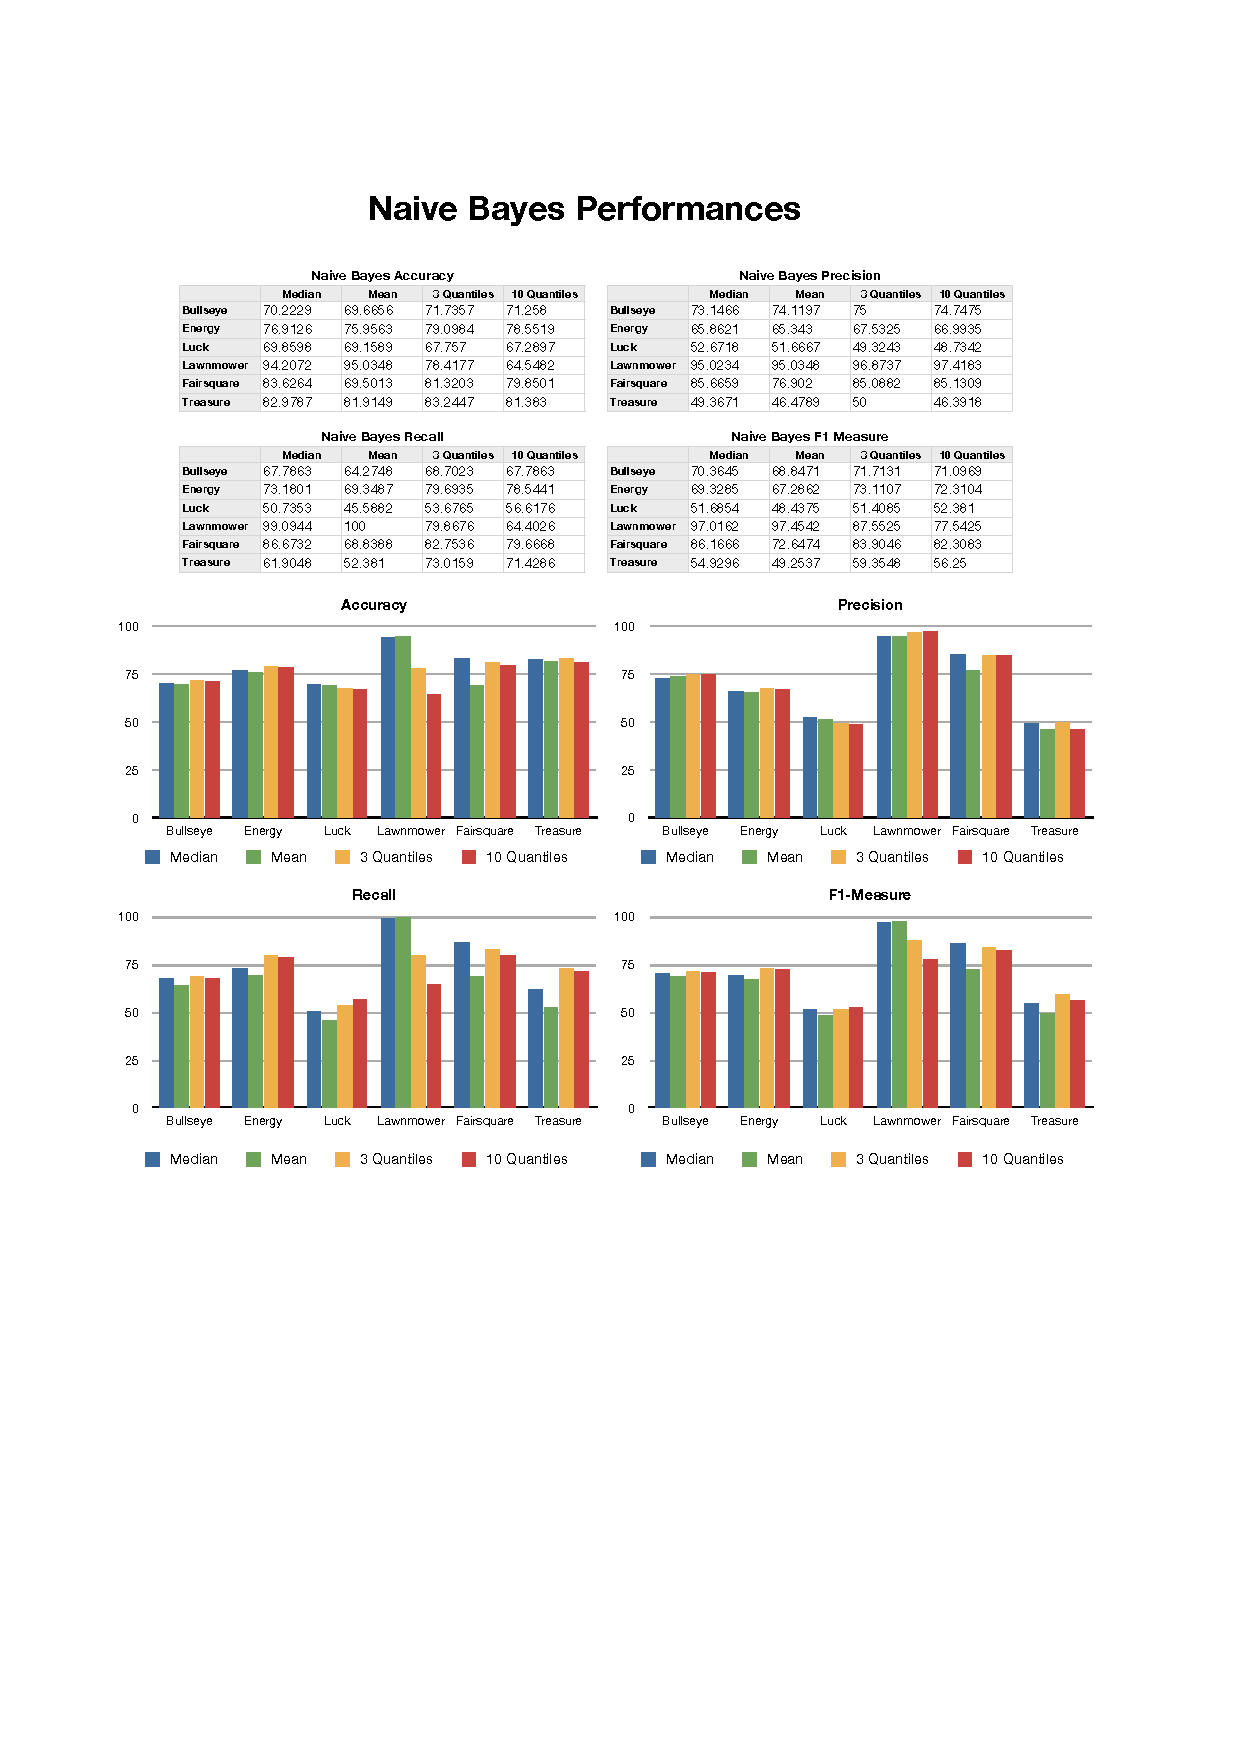
\includegraphics[width=\linewidth]{figures/NaiveBayes}
    \caption{Performance of the Naive Bayes classifier.%
      \label{fig:naivebayes}}
\end{figure}


%
\begin{figure}
    \centering
    \setlength{\tabcolsep}{0.0130\linewidth}
    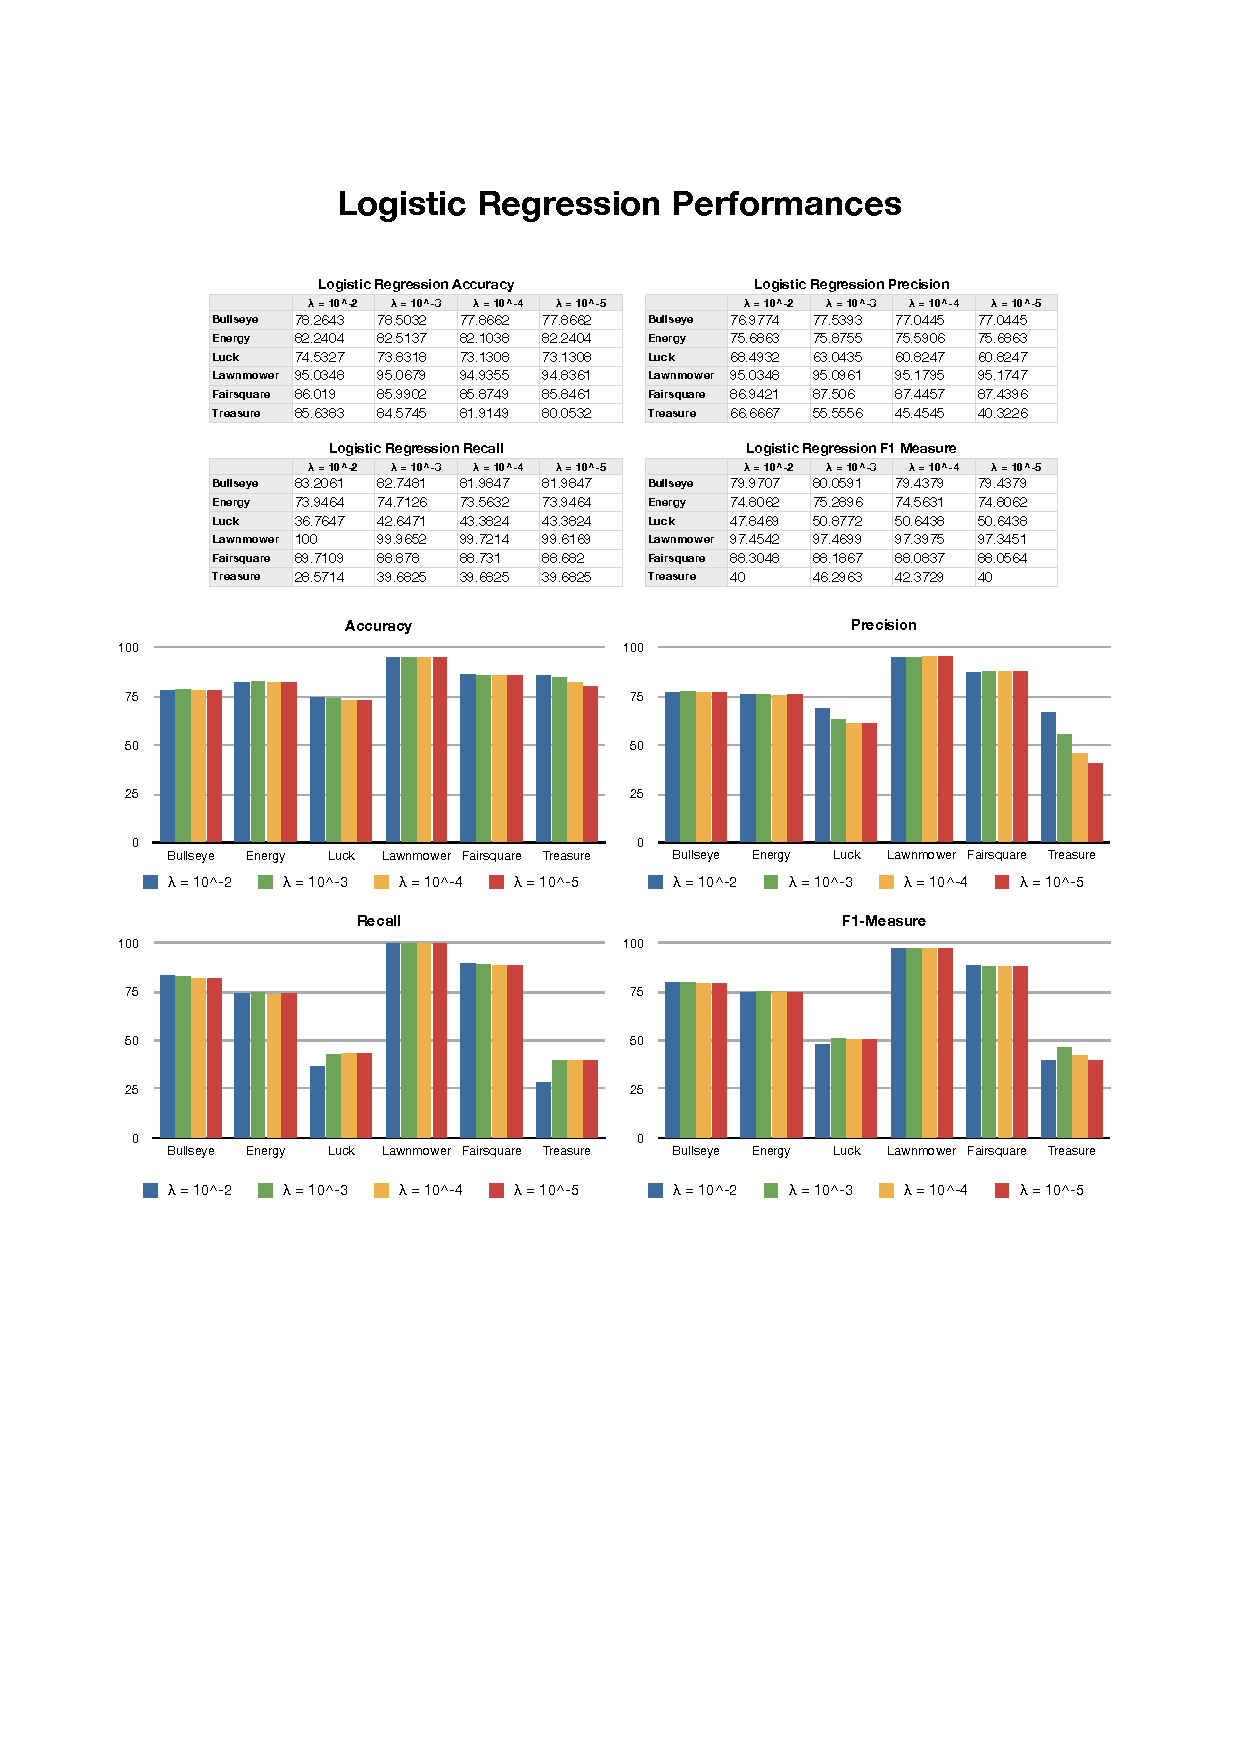
\includegraphics[width=\linewidth]{figures/LogisticRegression}
    \caption{Performance of the logistic regression classifier.%
      \label{fig:logisticregression}}
\end{figure}


%
\begin{figure}
    \centering
    \setlength{\tabcolsep}{0.0130\linewidth}
    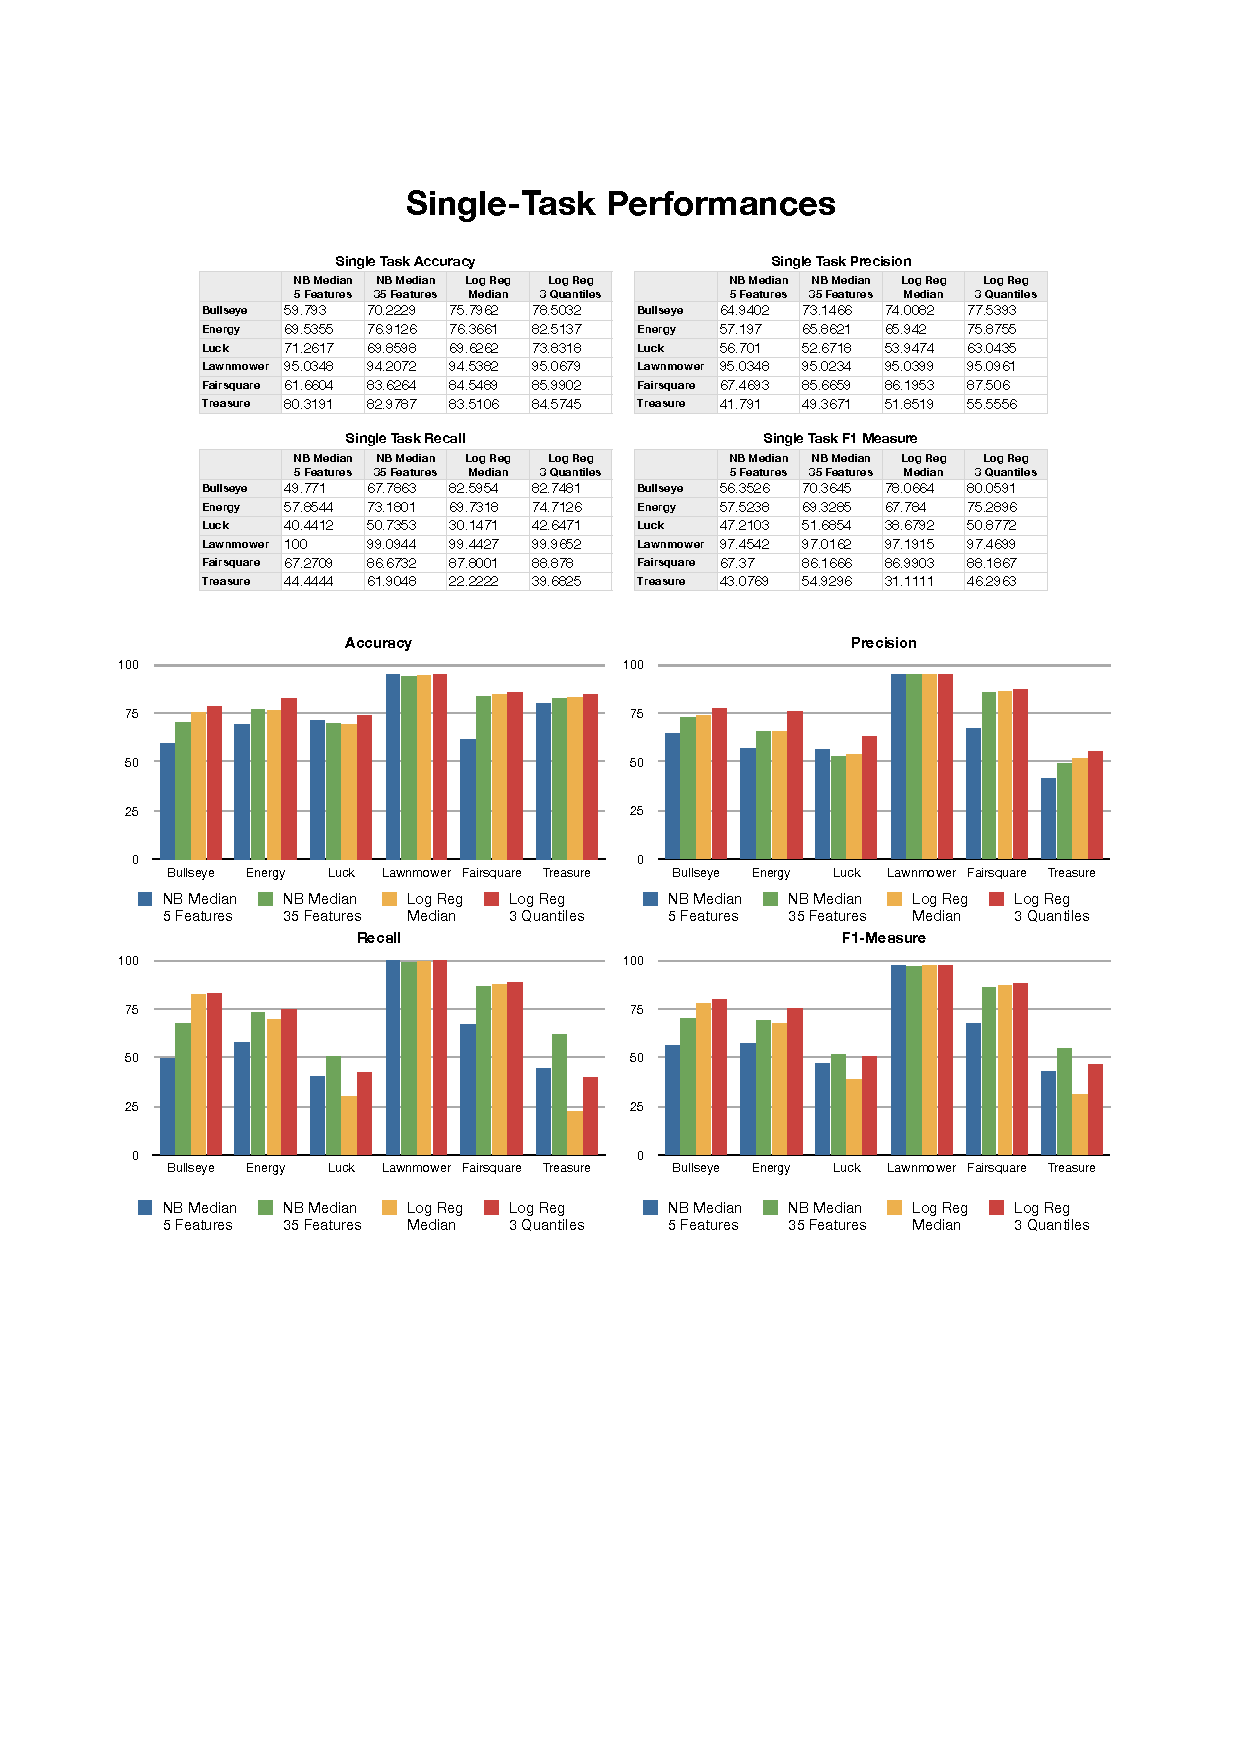
\includegraphics[width=\linewidth]{figures/SingleTask}
    \caption{Comparison of the various single-task classifiers.%
      \label{fig:singletask}}
\end{figure}


%
\begin{figure}
    \centering
    \setlength{\tabcolsep}{0.0130\linewidth}
    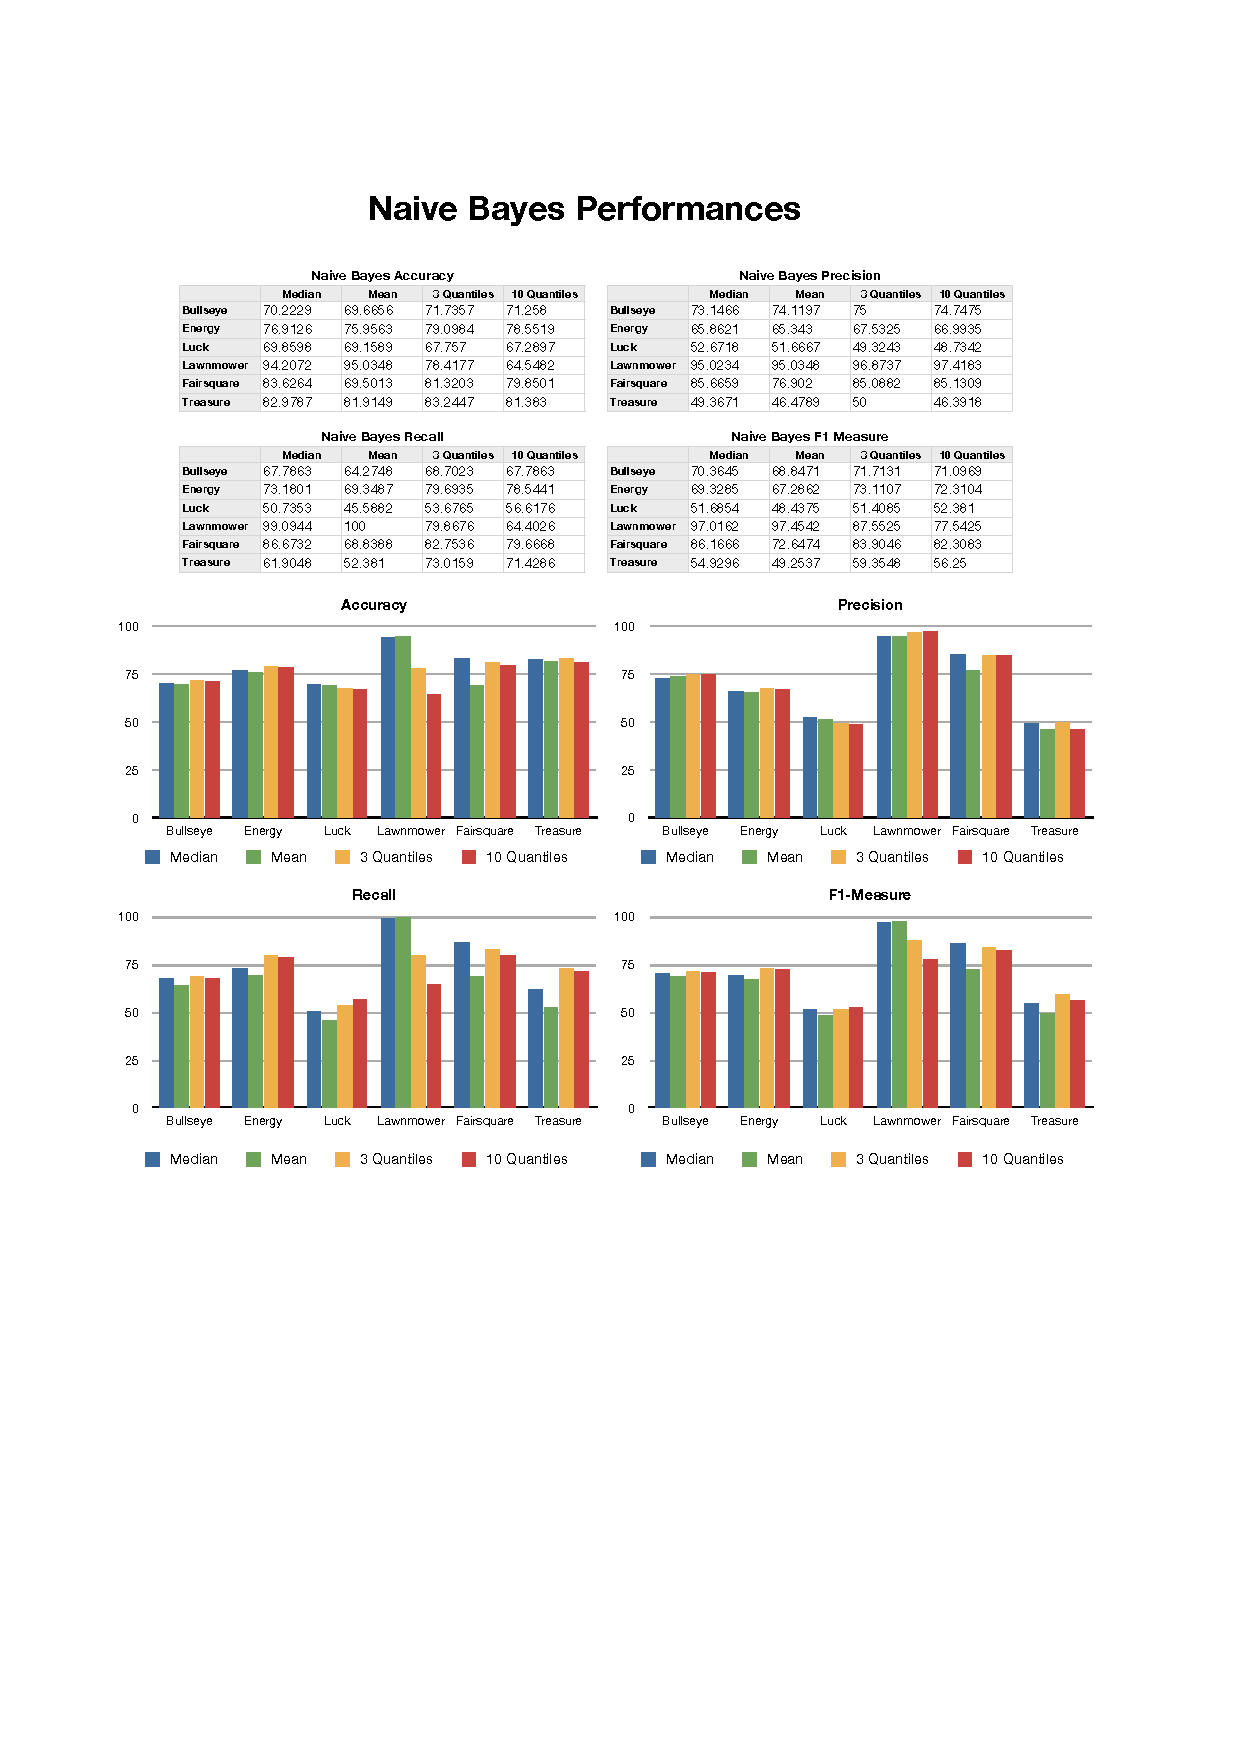
\includegraphics[width=\linewidth]{figures/NaiveBayes}
    \caption{Comparison of the various multi-task classifiers.%
      \label{fig:multitask}}
\end{figure}




